\documentclass[a4paper,12pt]{article}
\usepackage{maicoursework}

\usepackage[acronym, toc]{glossaries}

\usepackage{minted}

\begin{pycode}
import os

PROJECT_PATH = "/home/dmitry-vasiliev/WebstormProjects/db-course-project-app"

exclude = set([
    ".git",
    ".idea",
    "node_modules",
    "build"
])

exclude_file_ext = set([
    ".map",
    ".png",
    ".ico",
    ".jpeg",
    ".jpg",
])

exclude_filenames = set([
    "yarn.lock",
    ".env",
    "bundle.js",
    "site.webmanifest",
    ".gitignore",
    "config.ts"
])

ext_to_lang = {
    "handlebars": "html",
    "tsx": "jsx"
}
\end{pycode}

\setminted{
    fontsize=\scriptsize,
    baselinestretch=1,
    breaklines,
    linenos,
    numbersep=5pt,
    frame=lines
}
\makeatletter
\AtBeginEnvironment{noerr}{\dontdofcolorbox}
\def\dontdofcolorbox{\renewcommand\fcolorbox[4][]{##4}}
\makeatother
\newenvironment{noerr}{}

\makeglossaries

\newacronym{api}{API}{Applicatoin Programming Interface}
\newacronym{rest}{REST}{Representational State Transfer}
\newacronym{spa}{SPA}{Single Page Application}
\newacronym{mvp}{MVP}{Model View Presenter}
\newacronym{orm}{ORM}{Object-Relational Mapping}
\newacronym{jwt}{JWT}{JSON Web Token}
\newacronym{json}{JSON}{JavaScript Object Notaion}
\newacronym{bem}{BEM}{Block Element Modificator}
\newacronym{nosql}{NoSQL}{Not only SQL}

%%% Преамбула
\author{Васильев Дмитрий Олегович}
\title{Веб-приложение для тестирования}
\date{\today}
\MAIProfessorName{Романенков Александр Михайлович}
\MAIWorkType{Курсовой проект}
\MAISubject{Базы данных}

\begin{document}

\maketitle

\tableofcontents

\clearpage

\printglossaries

\clearpage

% Импортируем все секции
\section{Введение}

\subsection{Формальные требования}
\begin{enumerate}
    \item Необходимо выбрать предметную область для создания базы данных. Выбранная предметная область должна быть уникальной для всего потока, а не только в рамках учебной группы.
    \item Необходимо описать таблицы и их назначение. Выполнить проектирование логической структуры базы данных. Описать схему базы данных. Все реальные таблицы должны иметь 3 нормальную форму или выше. База данных должна иметь минимум 5 таблиц.
    \item Необходимо разработать два клиентских приложения для доступа к базе данных. Данные приложения должны быть написаны на двух разных языках программирования и иметь разный интерфейс (например, классическое оконное приложение и web-приложение). Выбор языков программирования произволен: C/C++, python, perl, ruby, JavaScript, php, swift, C\# 5.0, Java и др.
    \item Необходимо организовать различные роли пользователей и права доступа к данным. Далее, необходимо реализовать возможность создания архивных копий и восстановления данных из клиентского приложения.
    \item При разработке базы данных следует организовать логику обработки данных не на стороне клиента, а, например, на стороне сервера, базы данных, клиентские приложения служат только для представления данных и тривиальной обработки данных.
    \item Ваша база данных должна иметь представления, триггеры и хранимые процедуры, причем все эти объекты должны быть осмысленны, а их использование оправдано.
    \item При показе вашего проекта необходимо уметь демонстрировать таблицы, представления, триггеры и хранимые процедуры базы данных, внешние ключи, ограничения целостности и др. В клиентских приложениях уметь демонстрировать подключение к базе данных, основные режимы работы с данными (просмотр, редактирование, обновление \dots)
    \item Необходимо реализовать корректную обработку различного рода ошибок, которые могут возникать при работе с базой данных.
\end{enumerate}

\subsection{Предметная область}


\subsection{Стэк технологий}
\begin{itemize}
    \item \textcite{wiki:js} --- мультипарадигменный язык программирования. Поддерживает объектно-ориентированный, императивный и функциональный стили. Является реализацией стандарта \textcite{wiki:es}.
    \item \textcite{wiki:css} --- формальный язык описания внешнего вида документа, написанного с использованием языка разметки.
    \item \textcite{wiki:html} --- гипертекстовый язык разметки.
    \item \textcite{node.js} --- среда выполнения JavaScript, созданная на основе движка Chrome V8 JavaScript.
    \item \textcite{express} --- минимальный и гибкий \textcite{node.js} фреймворк для создания веб-приложений.
    \item \textcite{python} --- язык программирования, который позволяет быстро работать и более эффективно интегрировать системы.
    \item \textcite{postgres} --- объектно-реляционная база данных с открытым исходным кодом.
\end{itemize}
\clearpage
\section{Инфраструктура проекта}

\subsection{Архитекрутра}
За основу берётся архитектурный паттерн \acrshort{mvc}. Он предполагает разделение данных приложения, пользовательского интерфейса и управляющей логики на три отдельных компонента: Модель, Представление и Контроллер – таким образом, что модификация каждого компонента может осуществляться независимо.

\begin{figure}[h]
    \begin{center}
        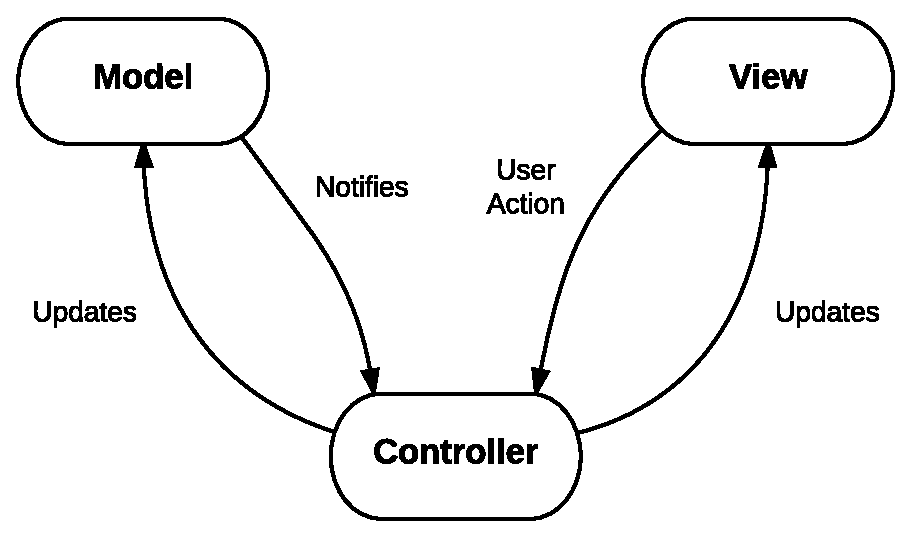
\includegraphics[scale=0.7]{images/MVC-basic.eps}
    \end{center}
    \caption{Визуализация архитектуры \acrshort{mvc}}
\end{figure}

\subsubsection{Связь логических компонетов и применяемых технологих}
\begin{itemize}
    \item Model --- \textcite{seqorm} для сервера и \textcite{redux} для клиента.
    \item View --- \textcite{react}
    \item Controller --- \textcite{express}
\end{itemize}

\subsection{Сущности}
Всегда перед проектированием проекта описывают сущности и их атрибуты. На основе данной информации будет стоится база данных. В моём случае они следующие:

\begin{itemize}
    \item Пользователь
    \begin{itemize}
        \item ID пользователя
        \item Логин
        \item Пароль
        \item Email
    \end{itemize}
    \item Тест
    \begin{itemize}
        \item ID теста
        \item Название
        \item Теги
        \item Контент
        \item Ответы
        \item Дата создания
        \item Дата последнего изменения
    \end{itemize}
    \item Тег
    \begin{itemize}
        \item ID тега
        \item Название
    \end{itemize}
    \item Попытка
    \begin{itemize}
        \item ID попытки
        \item ID пользователя
        \item ID теста
        \item Результат
        \item Ответы пользователя
        \item Дата прохождения
        \item Время прохождения
    \end{itemize}
\end{itemize}

\subsection{Сборка и запуск}
Все процессы отвечающие за сборку и запуск приложения я разделил на подзадачи. Каждая такая подзадача является npm скриптом. Они все описываются в файле package.json. Также среди данных скриптов можно выделить две группы -- Development и Production.

\subsubsection{Development}
Скрипты из данной группы отвечают за то, чтобы приложение можно было запускать в режиме разработки, а именно:
\begin{enumerate}
    \item сборка клинтской части не занимало слишком много времени
    \item клинет пересобирался при изменении какого-либо файла
    \item сервер перезапускался при изменения кода серверверной части
    \item в браузере были доступны source map
\end{enumerate}

\subsubsection{Production}


\subsection{Деплоинг}


\subsection{Организация работы с \textcite{git}}
\subsubsection{Git Workflow}
Для организации работы с системой контроля версий в проекте используется подход Git Workflow. Он нужен для согласованного и продуктивного выполнения работы.

\begin{figure}[h!]
    \begin{center}
        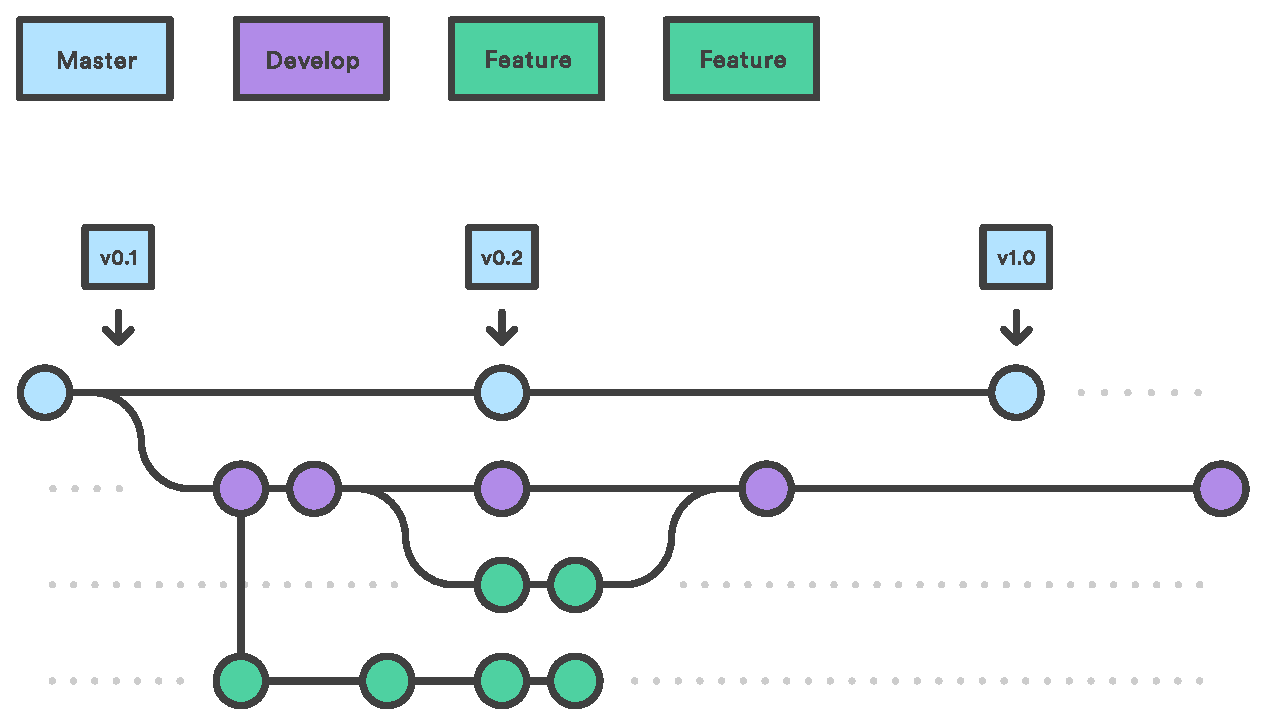
\includegraphics[scale=0.6]{images/git-workflow.eps}
    \end{center}
    \caption{Пример использования подхода Git Workflow}
\end{figure}

\subsubsection{Git hooks}
Чтобы в репозитории хранился код, который проходит проверки линтеров и тестовых фреймворков, нужно использовать Git Hooks. Они позволяют обработать события pre-commit, pre-push, post-commit и так далее.

Есть удобный пакет в npm -- husky. Он позволяет определить в package.json обработку событий. В моём проекте нужно, чтобы на событие pre-commit выполняли проверки линтеры, а потом при успешном результате исполнялись unit-тесты.

\begin{listing}[h!]
\begin{pycode}
import json
from pprint import pprint

with open(f"{PROJECT_PATH}/package.json", "r") as f:
    config = json.load(f)

    print(r"\begin{noerr}")
    print(r"\begin{minted}{json}")
    pprint(config["husky"])
    print(r"\end{minted}")
    print(r"\end{noerr}")
\end{pycode}
\caption{Настройки для Git Hooks}
\end{listing}

\clearpage
\section{Описание проекта}
\subsection{Разработка дизайна}
Так как я не дизайнер, то мне нужно оперировать концептами и эскизами интерфейса. Поэтому вначале я сделал макет страниц и связь между ними.

\subsection{Авторизации через \acrfull{jwt}}

\subsubsection{Авторизация}
\textbf{Авторизация} --- это процесс предоставления определённому лицу или группе лиц прав на выполнение определённых действий. Также сюда входит проверка данных, прав при попытке выполнения этих действий.

\subsubsection{Аутентификация}
\textbf{Аутентификация} --- процедура проверки подлинности данный.

\subsubsection{\acrfull{jwt}}
\begin{figure}[h!]
    \begin{center}
        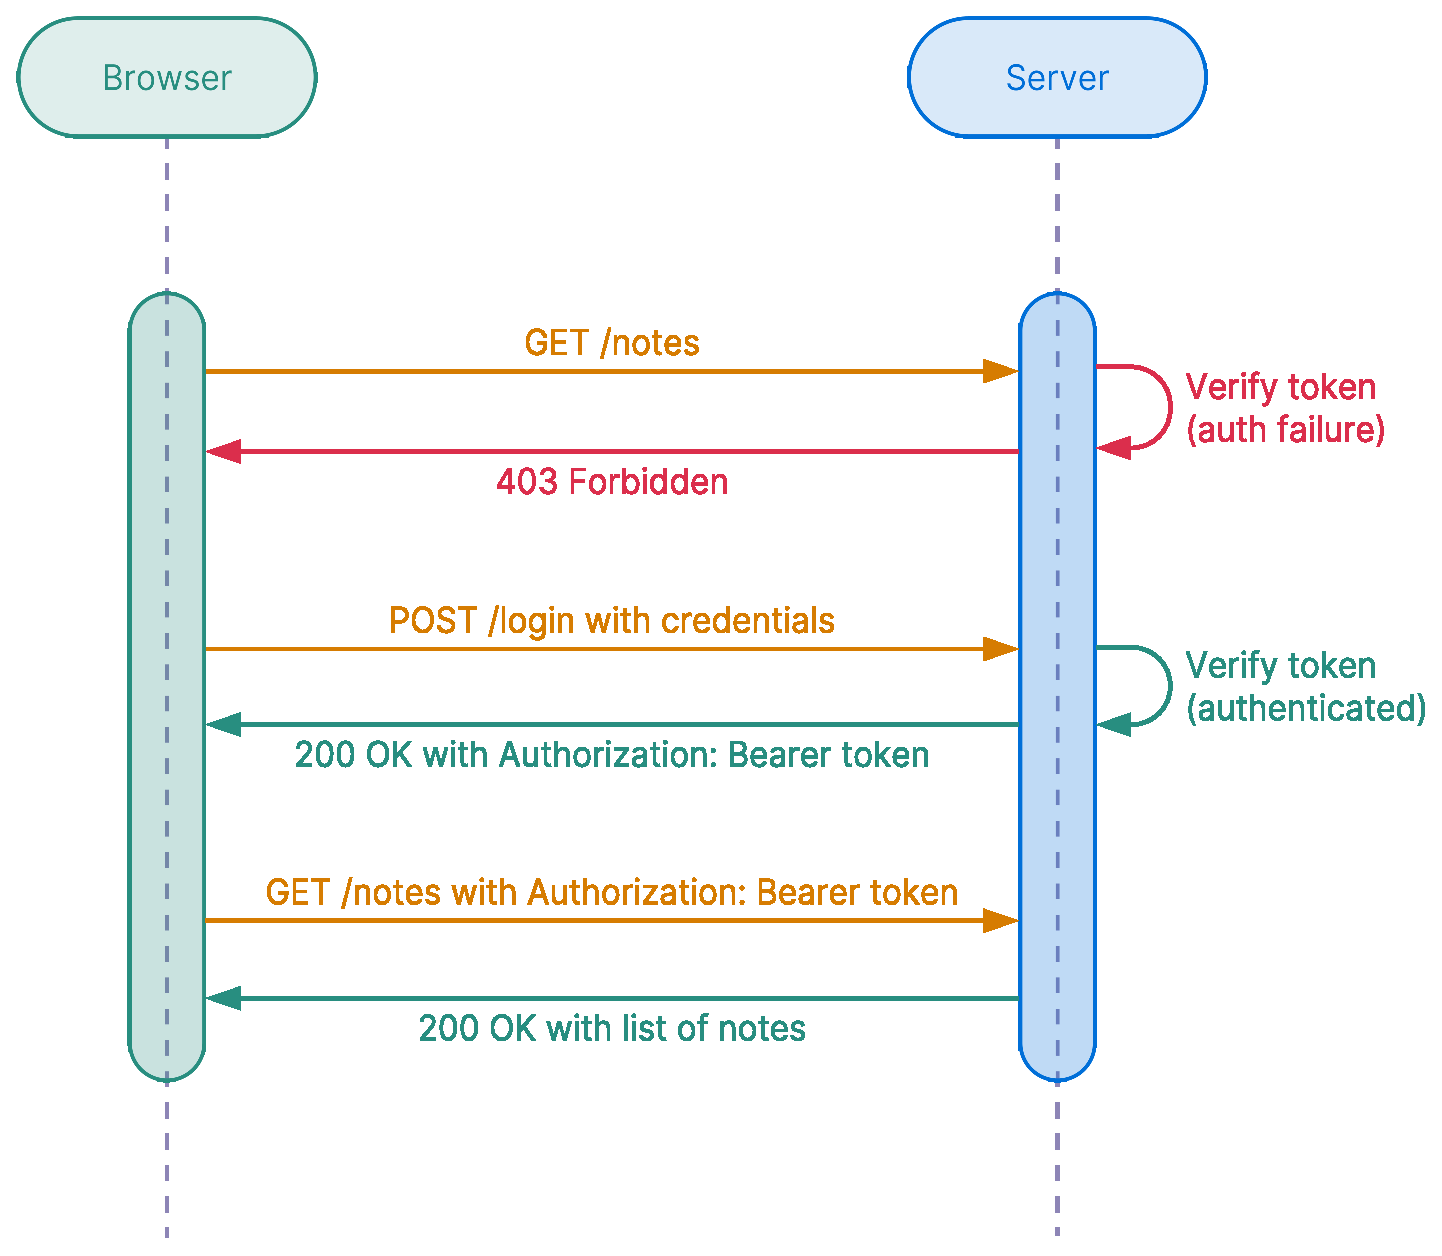
\includegraphics[scale=0.4]{images/jwt-example.eps}
        \caption{Демонстрация работы \acrshort{jwt}}
    \end{center}
\end{figure}

\textbf{\acrfull{jwt}} --- это открытый стандарт \href{https://tools.ietf.org/html/rfc7519}{(RFC 7519)}, который определяет способ для безопасной передачи информации между сторонами с помощью \acrshort{json} объектов. Эту информацию можно проверить, потому что она имеет цифровую подпись.

Вот несколько сценариев, в которых полезен \acrshort{jwt}:
\begin{itemize}
    \item \textbf{Авторизация} --- это наиболее распространенный сценарий использования \acrshort{jwt}. После того, как пользователь вошел в систему, каждый последующий запрос будет включать \acrshort{jwt}, позволяя пользователю получать доступ к маршрутам, службам и ресурсам, разрешенным с помощью этого токена.
    \item \textbf{Обмен информацией} --- \acrshort{jwt} хороший способ безопасной передачи информации между сторонами. Поскольку \acrshort{jwt} могут быть подписаны, например, с использованием пар открытого и закрытого ключей, вы можете быть уверены, что отправители являются теми, кем они себя называют. Кроме того, поскольку подпись рассчитывается с использованием \textbf{заголовка} и \textbf{полезных данных}, вы также можете убедиться, что содержимое не было изменено.
\end{itemize}

\acrshort{jwt} состоит из следующих частей:
\begin{itemize}
    \item \textbf{Заголовок} ---  содержит информацию о том, как должна вычисляться подпись. Обычно состоит из двух частей: типа токена, которым является \acrshort{jwt}, и используемого алгоритма подписи, такого как HMAC SHA256 или RSA.
    \item \textbf{Полезные данные} --- это данные, которые хранятся внутри \acrshort{jwt}. Они также называют JWT-claims (заявки). Список доступных полей для \acrshort{jwt} доступен на \href{https://en.wikipedia.org/wiki/JSON_Web_Token#Standard_fields}{Wiki}.
    \item \textbf{Подпись} --- используется для проверки того, что сообщение не было изменено в процессе. В компактной форме \acrshort{jwt} является сторой, которая состоит из трех частей, разделенных точками. Псевдокод вычисления подписи:
    \begin{noerr}
    \begin{minted}{js}
SECRET_KEY = 'some string';
unsignedToken = encodeBase64Url(header) + '.' + encodeBase64Url(payload)
signature = SHA256(unsignedToken, SECRET_KEY);

// собираем всё вместе
jwt = encodeBase64Url(header) + '.' + encodeBase64Url(payload) + '.' + encodeBase64Url(signature);
    \end{minted}
    \end{noerr}
\end{itemize}

\subsubsection{Реализация}
Авторизация проходит следущим образом:
\begin{enumerate}
    \item Пользователь делает \mintinline{text}{POST /api/signup} запрос на регистрацию. Если всё нормально, то в базе данных создаётся запись с данными пользователя.
    \item Пользователь делает \mintinline{text}{POST /api/signin} запрос на аутентификацию. Если данные верные, то высылается \acrshort{jwt} вместе с состоянием пользователя (логин, почта). Когда ответ с сервера получен, то \acrshort{jwt} сохраняется в localStorage (долговременное хранилище), а состояние передается в глобальное \textcite{redux} хранилище.
    \item После того, как состояние глобального хранилища обновилось, приложение обновляет интерфейс.
\end{enumerate}

Если перезагрузить веб-страницу, то \textcite{redux} хранилище обнуляется. Поэтому нам нужно сделать следующее: при запуске приложения проверять на валидность JWT, который лежит в localStorage. Это делается через \mintinline{text}{POST /api/init} запрос. Если токен валидный, то переавторизовываем пользователя. Иначе перенаправляем на главную страницу.

Далее этот токет будет использоваться для доступа к защищёнными ресурсам.

\subsection{Схема базы данных}
\begin{figure}[h!]
    \begin{center}
        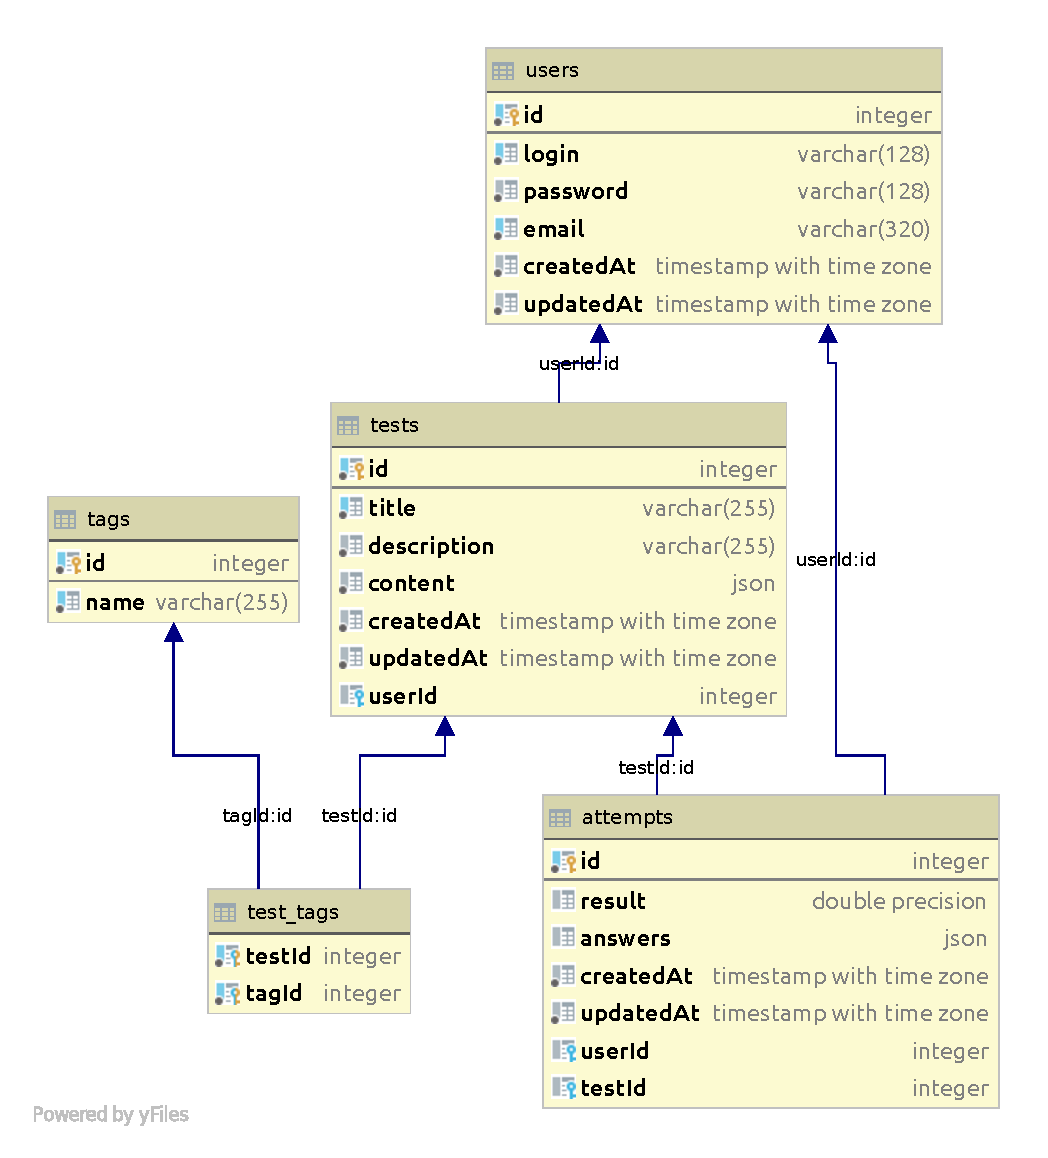
\includegraphics[scale=0.6]{images/db_scheme.eps}
    \end{center}
    \caption{Схема базы данных}
\end{figure}

\clearpage
\section{Заключение}
Благодаря данному курсовому проекту, я поверхностно освоил разработку \acrshort{spa} приложений с помощью библиотеки \textcite{react} и фреймворка \textcite{express}.

\subsection{Недостатки}
Подводя итоги, мне бы хотелось перечислить вещи, на которые я буду обращать внимание при разработке следующих проектов:
\begin{itemize}
    \item Использование CI/CD.
    \item Использование методологий в вёрстке. Например, \acrfull{bem}. Её разработали внутри компании Яндекс. У них есть свой стек технологий под данную методологию, который облегчает разработку клиентской части.
    \item Использование \acrshort{nosql} баз данных вместе с реалиционными. Хранить \acrshort{json} в таблице плохо, поэтому для этой задачи подходить \textcite{mongodb}.
    \item Разделение клиентского кода на чанки.
    \item Микросервисная архитектура.
\end{itemize}

\clearpage

\appendix
\section{Визуализации структуры проекта}
\begin{pycode}
import os

PROJECT_PATH = "/home/dmitry-vasiliev/WebstormProjects/db-course-project-app"

exclude = set([
    ".git",
    ".idea",
    "node_modules",
    "build"
])

print(r'\begin{verbatim}')

level_str = '---'
for root, dirs, files in os.walk(PROJECT_PATH):
    dirs[:] = [d for d in dirs if d not in exclude]
    path = root.split(os.sep)[4:]
    len_path = len(path)
    print(f"{(len_path - 1) * level_str} /{os.path.basename(root)}")

    for file in files:
        print(f"{len_path * level_str} {file}")

print(r'\end{verbatim}')
\end{pycode}

\clearpage
\section{Код проекта}
\begin{pycode}
exclude_file_ext = set([
    ".map",
    ".png",
    ".ico",
    ".jpeg",
    ".jpg",
])

exclude_filenames = set([
    "yarn.lock",
    ".env",
    "bundle.js",
    "site.webmanifest",
    ".gitignore"
])

ext_to_lang = {
    "handlebars": "html",
    "tsx": "jsx"
}

for root, dirs, files in os.walk(PROJECT_PATH):
    dirs[:] = [d for d in dirs if d not in exclude]
    relative_path = root.split(os.sep)[4:]

    for file in files:
        if file in exclude_filenames:
                continue

        full_filename = os.path.join(root, file)
        relative_filename = os.path.join(os.sep.join(relative_path), file)
        _, file_extension = os.path.splitext(full_filename)
        lang = file_extension[1:]

        if file_extension in exclude_file_ext:
            continue

        if lang in ext_to_lang:
            lang = ext_to_lang[lang]

        if lang == '':
            lang = "text"

        print(r'\begin{verbatim}')
        print(relative_filename)
        print(r'\end{verbatim}')

        print(r"\begin{noerr}")
        print(r''.join([
            r"\inputminted[linenos,numbersep=5pt,frame=lines]",
            f"{{{lang}}}",
            f"{{{full_filename}}}"
        ]))
        print(r"\end{noerr}")
\end{pycode}

\clearpage

\printbibliography

\end{document}